% VUT FIT MITAI
% MSZ 2021/2022
% Author: Vladimir Dusek
% Login: xdusek27

%%%%%%%%%%%%%%%%%%%%%%%%%%%%%%%%%%%%%%%%%%%%%%%%%%%%%%%%%%%%%%%%%%%%%%%%%%%%%%%%

% Path to figures
\graphicspath{{msp/testy/figures}}

%%%%%%%%%%%%%%%%%%%%%%%%%%%%%%%%%%%%%%%%%%%%%%%%%%%%%%%%%%%%%%%%%%%%%%%%%%%%%%%%

\chapter{MSP~--~Vícevýběrové testy, testy o rozdělení, testy dobré shody.}

%%%%%%%%%%%%%%%%%%%%%%%%%%%%%%%%%%%%%%%%%%%%%%%%%%%%%%%%%%%%%%%%%%%%%%%%%%%%%%%%

\section{Zdroje}

\begin{compactitem}
    \item \path{MSP_pred_02_Opakovani_Statistika_Regrese.}pdf
    \item \path{MSP_pred_04_ANOVA.pdf}
    \item \path{MSP_pred_08_Testy_DS_Testy_rozdeleni.pdf}
    \item Wikipedia
\end{compactitem}

%%%%%%%%%%%%%%%%%%%%%%%%%%%%%%%%%%%%%%%%%%%%%%%%%%%%%%%%%%%%%%%%%%%%%%%%%%%%%%%%

\section{ANOVA}

\begin{compactitem}
    \item ANOVA (\textit{analysis of variance}, analýza rozptylu) jsou statistické metody, které umožňují provádět vícenásobné porovnávání středních hodnot (resp. rozptylů).

    \item V čem je rozdíl oproti základním testům hypotéz pro vybraná rozdělení?

    \begin{compactitem}
        \item ANOVA jsou souhrnné testy pro více něž dva výběry (proto spadá pod vícevýběrové testy).

        \item Proč neudělat více dvouvýběrových testů? Museli bychom v případě více jak 2 hodnot faktoru provést dvouvýběrový test pro všechny dvojice hodnot, nebo současně porovnat naměřené hodnoty s předem danou hodnotou (efektivita).
    \end{compactitem}

    \item ANOVA je založena na hodnocení vztahů mezi rozptyly porovnávaných výběrových souborů (testování shody středních hodnot se převádí na testování shody dvou rozptylů).

    \item \textbf{Faktor} -- Statistický znak (znaky), který ovlivňuje měřenou veličinu. U každého faktoru uvažujeme o konečném počtu jeho hodnot.  \begin{compactitem}
        \item Např. chov králíků, zajímá nás velikost (měřená veličina) v závislosti na typu krmiva (faktor).

        \item Např. Dva termíny pro písemku ze cvičení MSP. Zajímá nás počet bodů z písemky (měřená veličina), v závislosti na skupině (jeden faktor) a na termínu (druhý faktor).
    \end{compactitem}
\end{compactitem}

\subsection{Postup}

\paragraph*{1. Test středních hodnot}

\begin{compactitem}
    \item Testování hypotézy:
    $$ H : \mu_1 = \mu_2 = \ldots = \mu_n $$

    \item Dílčí kroky: \begin{compactitem}
        \item variabilita mezi skupinami,
        \item celkovou variabilita,
        \item součet variability uvnitř skupin.
    \end{compactitem}
\end{compactitem}

\paragraph*{2.) Post host analýza}

\begin{compactitem}
    \item Pokud analýza rozptylu zamítne nulovou hypotézu $ H : \mu_1 = \mu_2 = \ldots = \mu_n $ o vlivu působícího faktoru, je nutno doplnit rozbor ještě dalšími metodami následného zkoumání existujících rozdílů. Tyto tzv. multikomparativní testy (testy pro mnohonásobné porovnávání) pak dávají výsledkem statistickou významnost jednotlivých rozdílů středních hodnot u všech možných párů porovnávaných skupin.

    \item Obvykle testujeme tzv. kontrasty, tj. hledáme dvojice $A_i$ a $A_j$, které vliv třídícího znaku způsobují.

    \item Pro každou dvojici testujeme hypotézu $ H : \alpha_i = \alpha_j $ vzhledem k $ H : \alpha_i \not= \alpha_j $.

    \item Testy: \begin{compactitem}
        \item Scheffeho metoda (F-test)
    \end{compactitem}
\end{compactitem}

\paragraph*{3.) Test rovnosti rozptylů}

\begin{compactitem}
    \item Test rovnosti rozptylů (test homoskedasticity).

    \item Testujeme hypotézu
    $$ H : \sigma^2_1 = \sigma^2_2 = \ldots = \sigma^2_n $$

    \item Proti alternativní
    $$ H_A : \exists i, j : \sigma^2_i \not= \sigma^2_j $$

    \item Testy: \begin{compactitem}
        \item Barlettův test
    \end{compactitem}
\end{compactitem}

\subsection{Jednofaktorová ANOVA}

\begin{compactitem}
    \item Náhodná proměnná je ovlivněna pouze jedním faktorem.

    \item U náhodné veličiny $X$ uvažujeme jeden faktor $A$, který nabývá $I$ různých kvalitativních
    hodnot $A_1, A_2, \ldots, A_I$, kde $I > 2$. \begin{compactitem}

        \item Každá kvalitativní hodnota $A_i$ je popsána náhodnou veličinou $X_i$.

        \item Náhodné veličiny $X_1, X_2, \ldots, X_I$ jsou nezávislé.
    \end{compactitem}

    \item Testujeme hypotézu
    $$ H : \mu_1 = \mu_2 = \ldots = \mu_n $$

    \item Proti alternativní
    $$ H_A : \exists i, j : \mu_i \not= \mu_j $$
\end{compactitem}

\subsection{Dvoufaktorová ANOVA}

\begin{compactitem}
    \item V praxi se často setkáváme s pokusy, kdy sledujeme více působících faktorů, např. vliv krmení a plemene, vliv léku v různých stádiích onemocnění, vliv živné půdy a způsobu kultivace na růst zárodků, vliv různých druhů antibiotik a jejich dávky apod. Pokud zkoumáme vliv dvou a více faktorů působících na závisle proměnnou, hovoříme o vícefaktorové analýze rozptylu.

    \item Náhodná proměnná je ovlivněna dvěma (nebo více) faktory.

    \item Dvoufaktorová bez interakce -- náhodná proměnná je ovlivněna dvěma nezávislými faktory.

    \item Dvoufaktorová s interakcí -- náhodná proměnná je ovlivněna dvěma závislými faktory.
\end{compactitem}

%%%%%%%%%%%%%%%%%%%%%%%%%%%%%%%%%%%%%%%%%%%%%%%%%%%%%%%%%%%%%%%%%%%%%%%%%%%%%%%%

\section{Testy dobré shody a testy o rozdělení}

\paragraph*{Princip testů dobré shody}

\begin{compactitem}
    \item Testy dobré shody vycházejí z porovnání teoretické pravděpodobnosti a odhadnuté pravděpodobnosti pomocí relativních četností u náhodné veličiny, která může nabývat
    konečného počtu možností. \begin{compactitem}
        \item Odpovídají empirická data nějakému teoretickému rozdělení?
    \end{compactitem}

    \item Vychází se z Multinomického rozdělení, které definuje pravděpodobnost při výběru (s opakováním) z konečného počtu možností.
\end{compactitem}

\paragraph*{Testy o rozdělení}
\begin{compactitem}
    \item Nechť $X$ je náhodná proměnná, která má distribuční funkci $F(x, \theta)$. Předpokládejme, že neznáme tvar distribuční funkce (nevíme jaké má rozdělení) a neznáme parametr $\theta$. Na základě měření (pokusů) chceme odhadnou typ rozdělení a neznámý parametr $\theta$. Provedeme $n$ pokusů (měření). Výsledky těchto pokusů jsou popsány náhodným výběrem $X = ( X_1, \ldots, X_n )$ a jeho realizací $x = ( x_1 , \ldots, x_n )$.

    \item Opět předpokládáme, že složky náhodného vektoru jsou nezávislé a mají stejné rozdělení jako náhodná proměnná $X$.

    \item Při testování hypotéz o rozdělení si zvolíme rozdělení, s kterým chceme porovnat naměřená data. Pokud rozdělení obsahuje neznámý parametr, pro jeho odhad použijeme statistiky pro bodový odhad.

    \item Hypotéza je ve tvaru:
    $$ H : X \sim F ( x, \theta ) ~,~ H_A : X \not= F ( x, \theta ) $$

    \item Testy: \begin{compactitem}
        \item Pearsonův chí-kvadrát test ($\chi^2$),
        \item Kolmogorov-Smirnov,
        \item Anderson-Darling,
        \item grafické metody.
    \end{compactitem}
\end{compactitem}

%%%%%%%%%%%%%%%%%%%%%%%%%%%%%%%%%%%%%%%%%%%%%%%%%%%%%%%%%%%%%%%%%%%%%

\section{Příklad: Při kontrole výrobků byla sledována odchylka X [mm] jejich rozměru od požadované velikosti. Naměřené hodnoty tvoří statistický soubor.}

\begin{figure}[H]
    \centering
    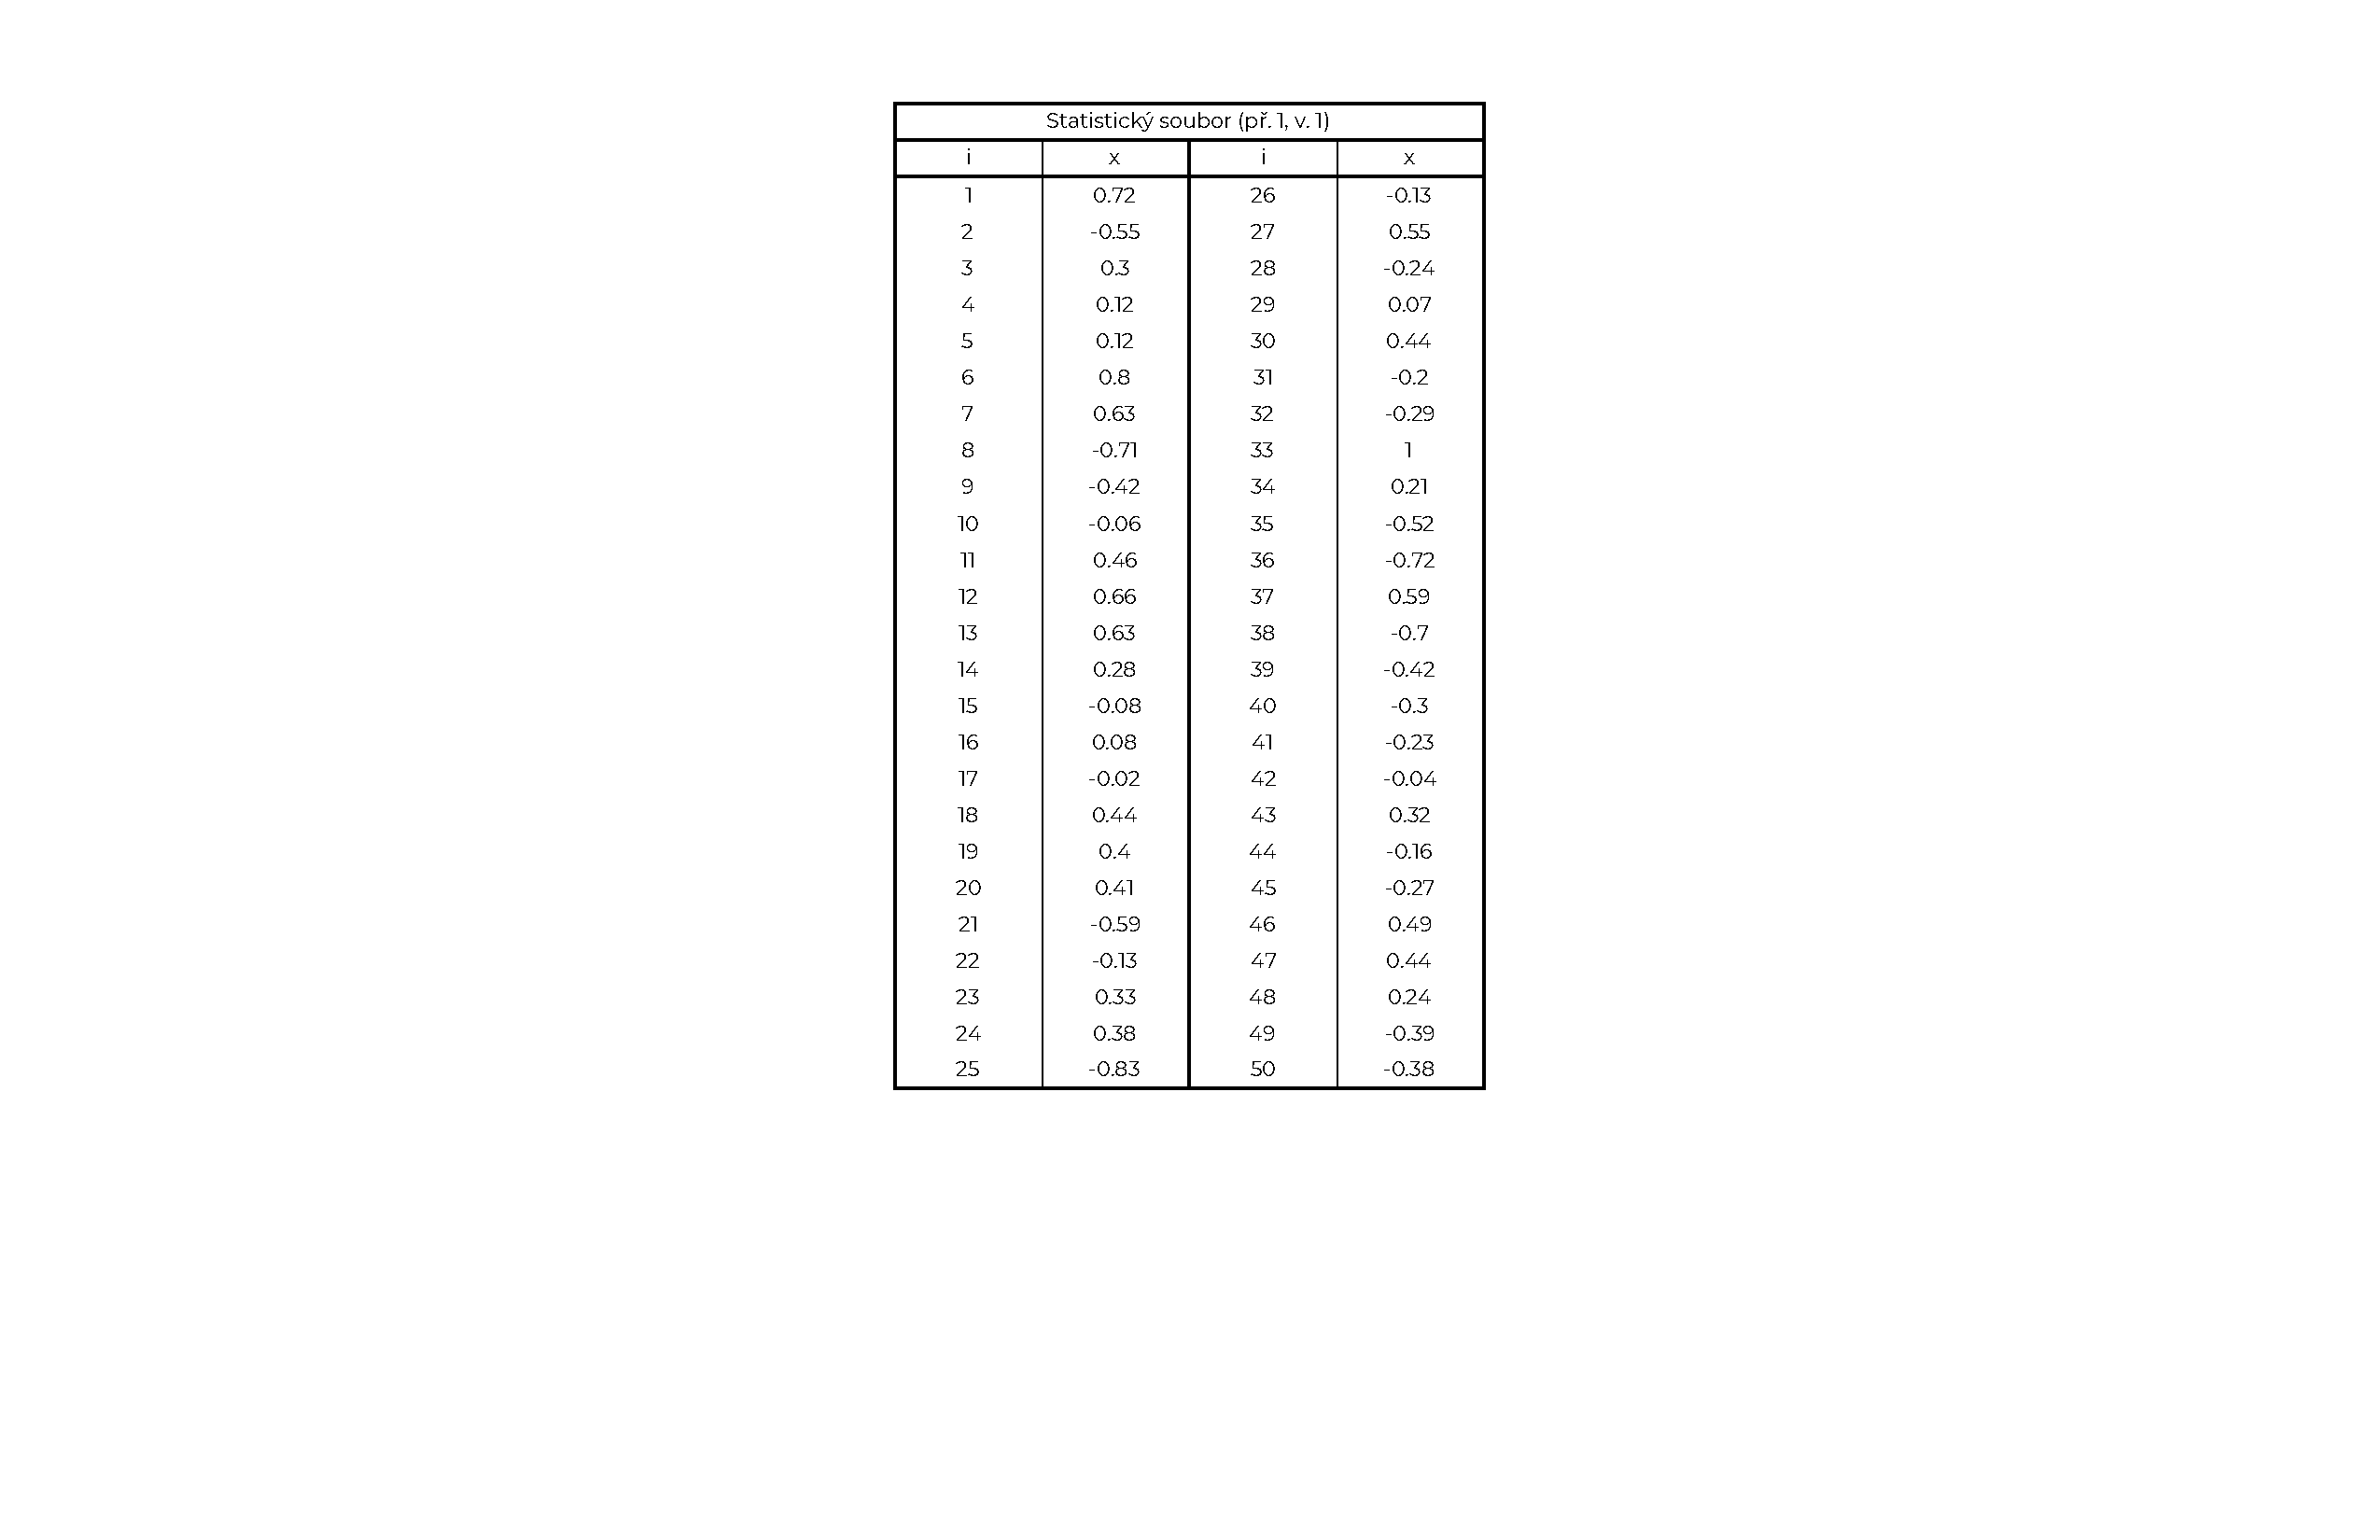
\includegraphics[width=.49\linewidth]{1-1-crop.pdf}
    \hfill
    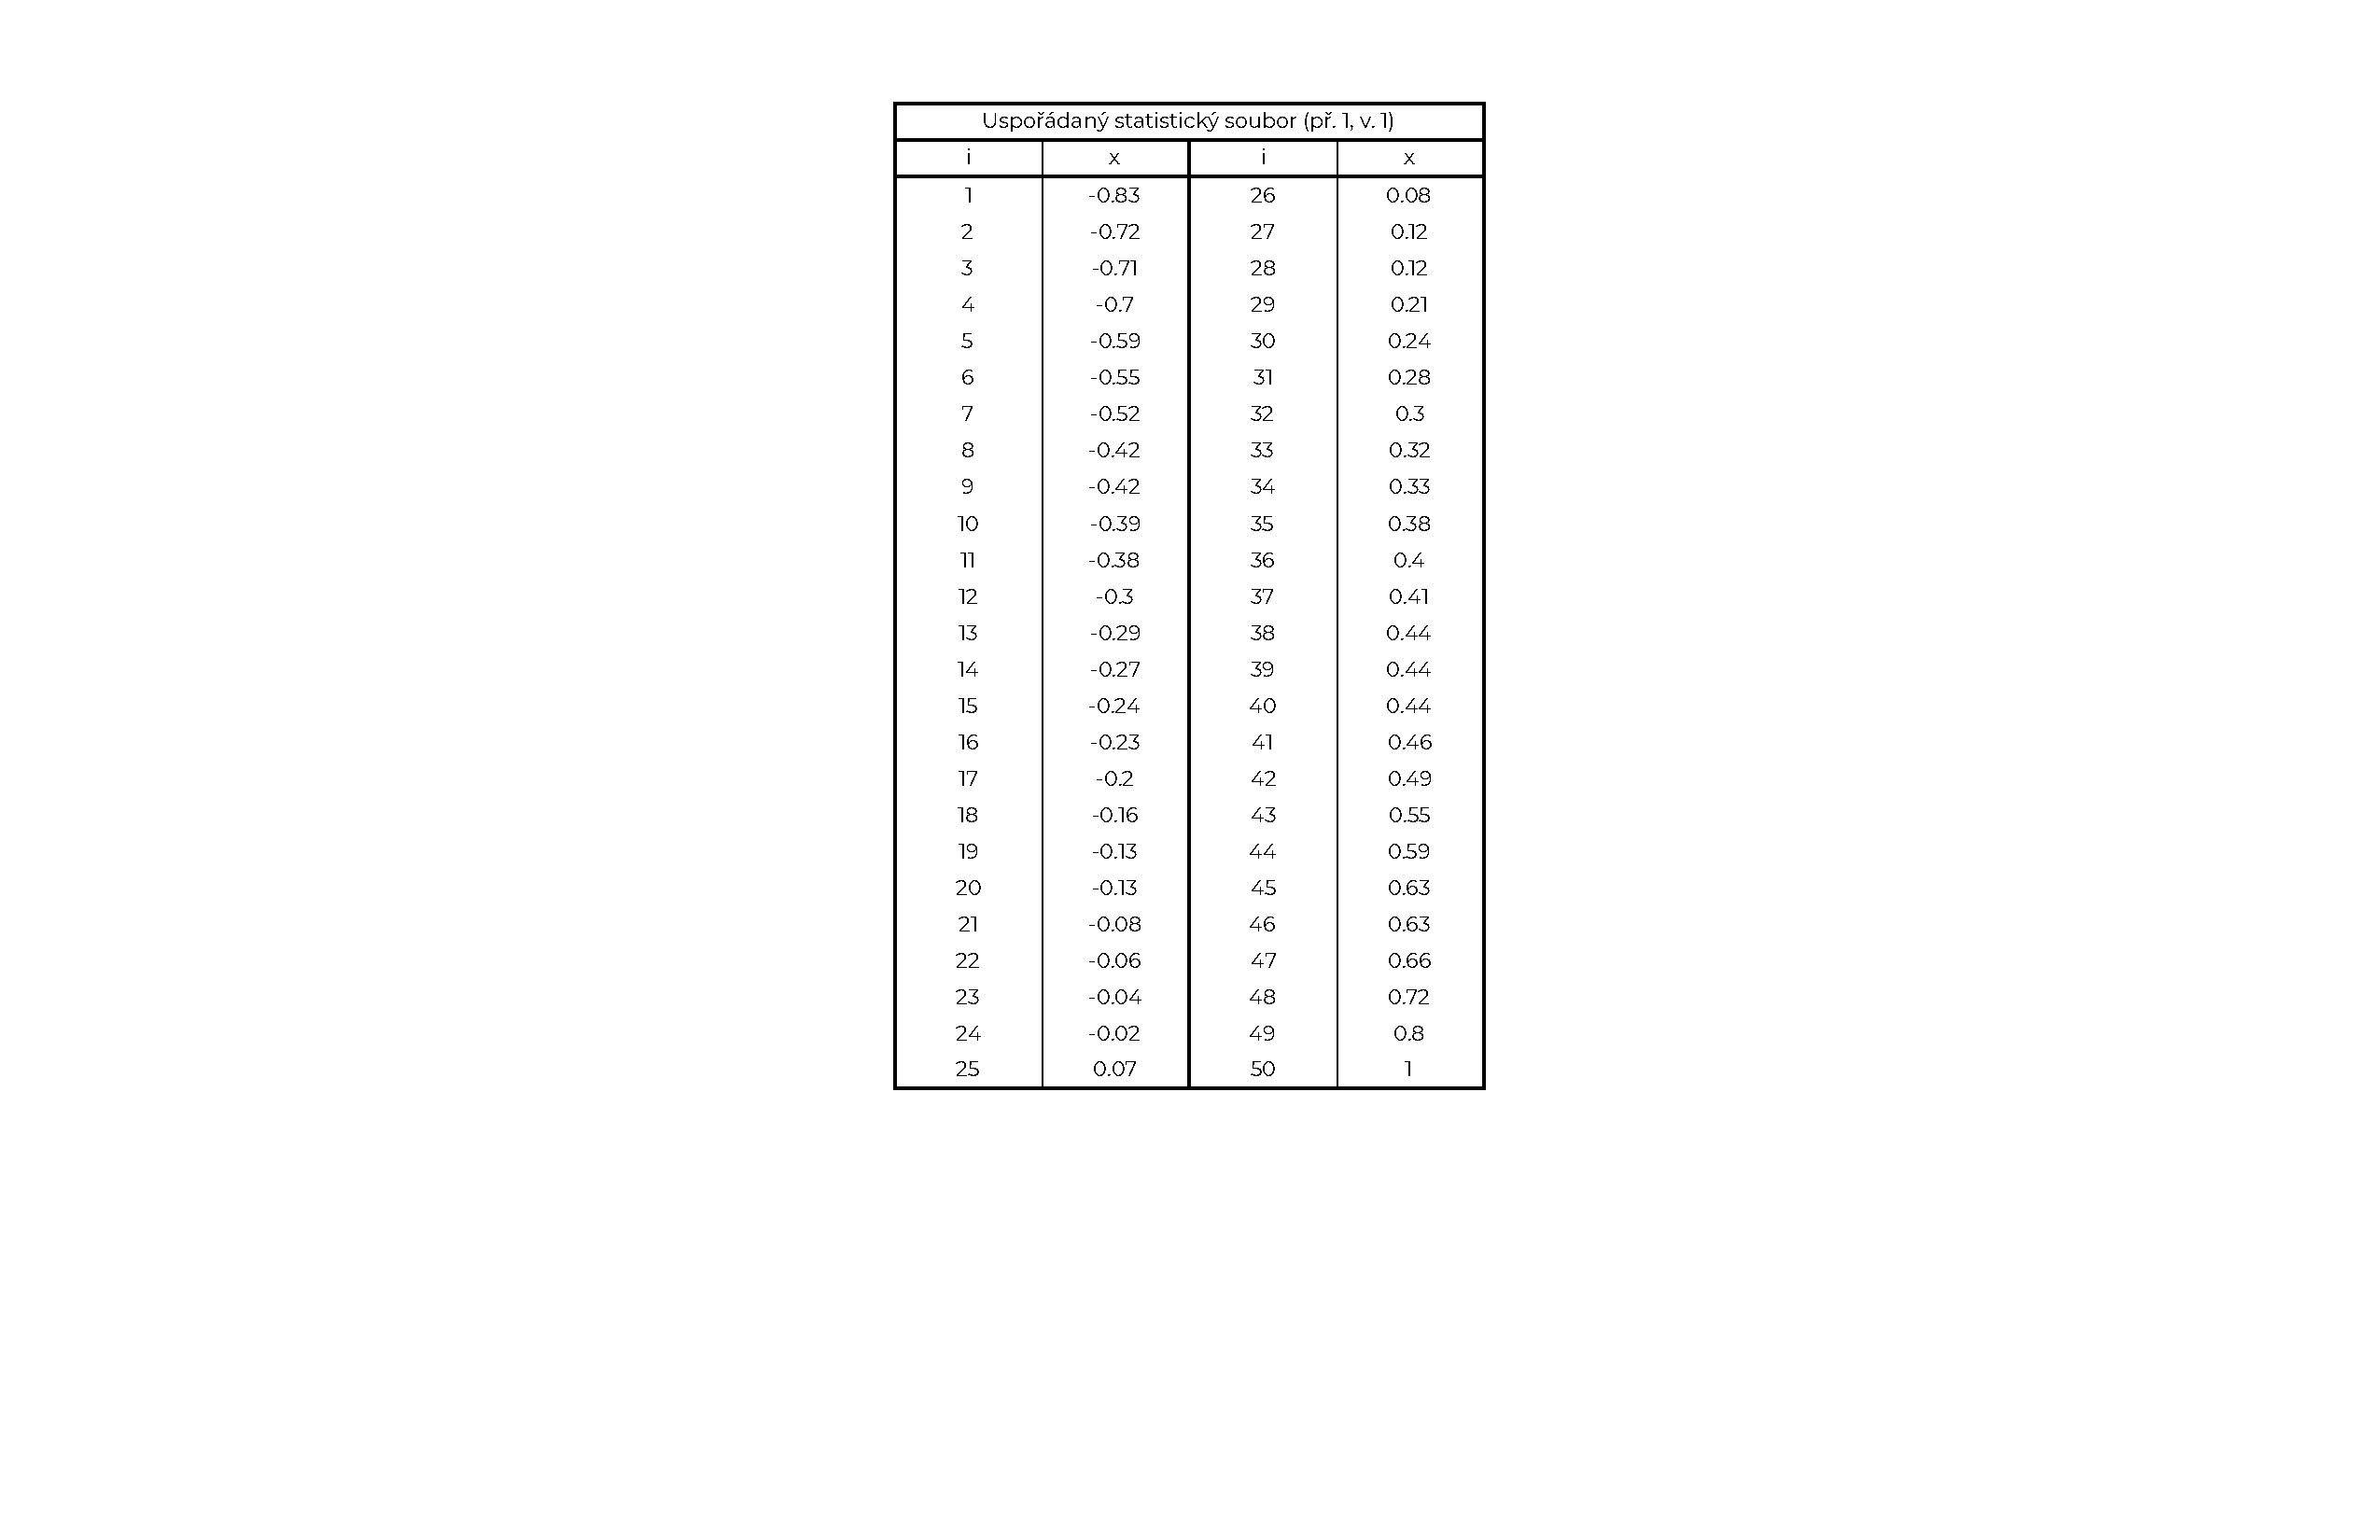
\includegraphics[width=.49\linewidth]{1-2-crop.pdf}
\end{figure}

%%%%%%%%%%%%%%%%%%%%%%%%%%%%%%%%%%%%%%%%%%%%%%%%%%%%%%%%%%%%%%%%%%%%%

\subsection{Proveďte roztřídění statistického souboru, vytvořte tabulku četností a nakreslete histogramy pro relativní četnosti a relativní kumulativní četnosti.}

\begin{compactitem}
    \item Variační obor:
    $${\displaystyle \big\langle x_{(1)} ~,~ x_{(n)} \big\rangle = \big\langle \min_{i} x_i ~,~ \max_{i} x_i \big\rangle = \big\langle -0.83 ~,~ 1 \big\rangle}$$

    \item Rozpětí:
    $${\displaystyle x_{(n)} - x_{(1)} = 1.83}$$

    \item Počet tříd:
    $${\displaystyle m = 10}$$

    \item Délka třídy:
    $${\displaystyle \frac{x_{(n)} - x_{(1)}}{m} = 0.183}$$
\end{compactitem}

\begin{figure}[H]
    \centering
    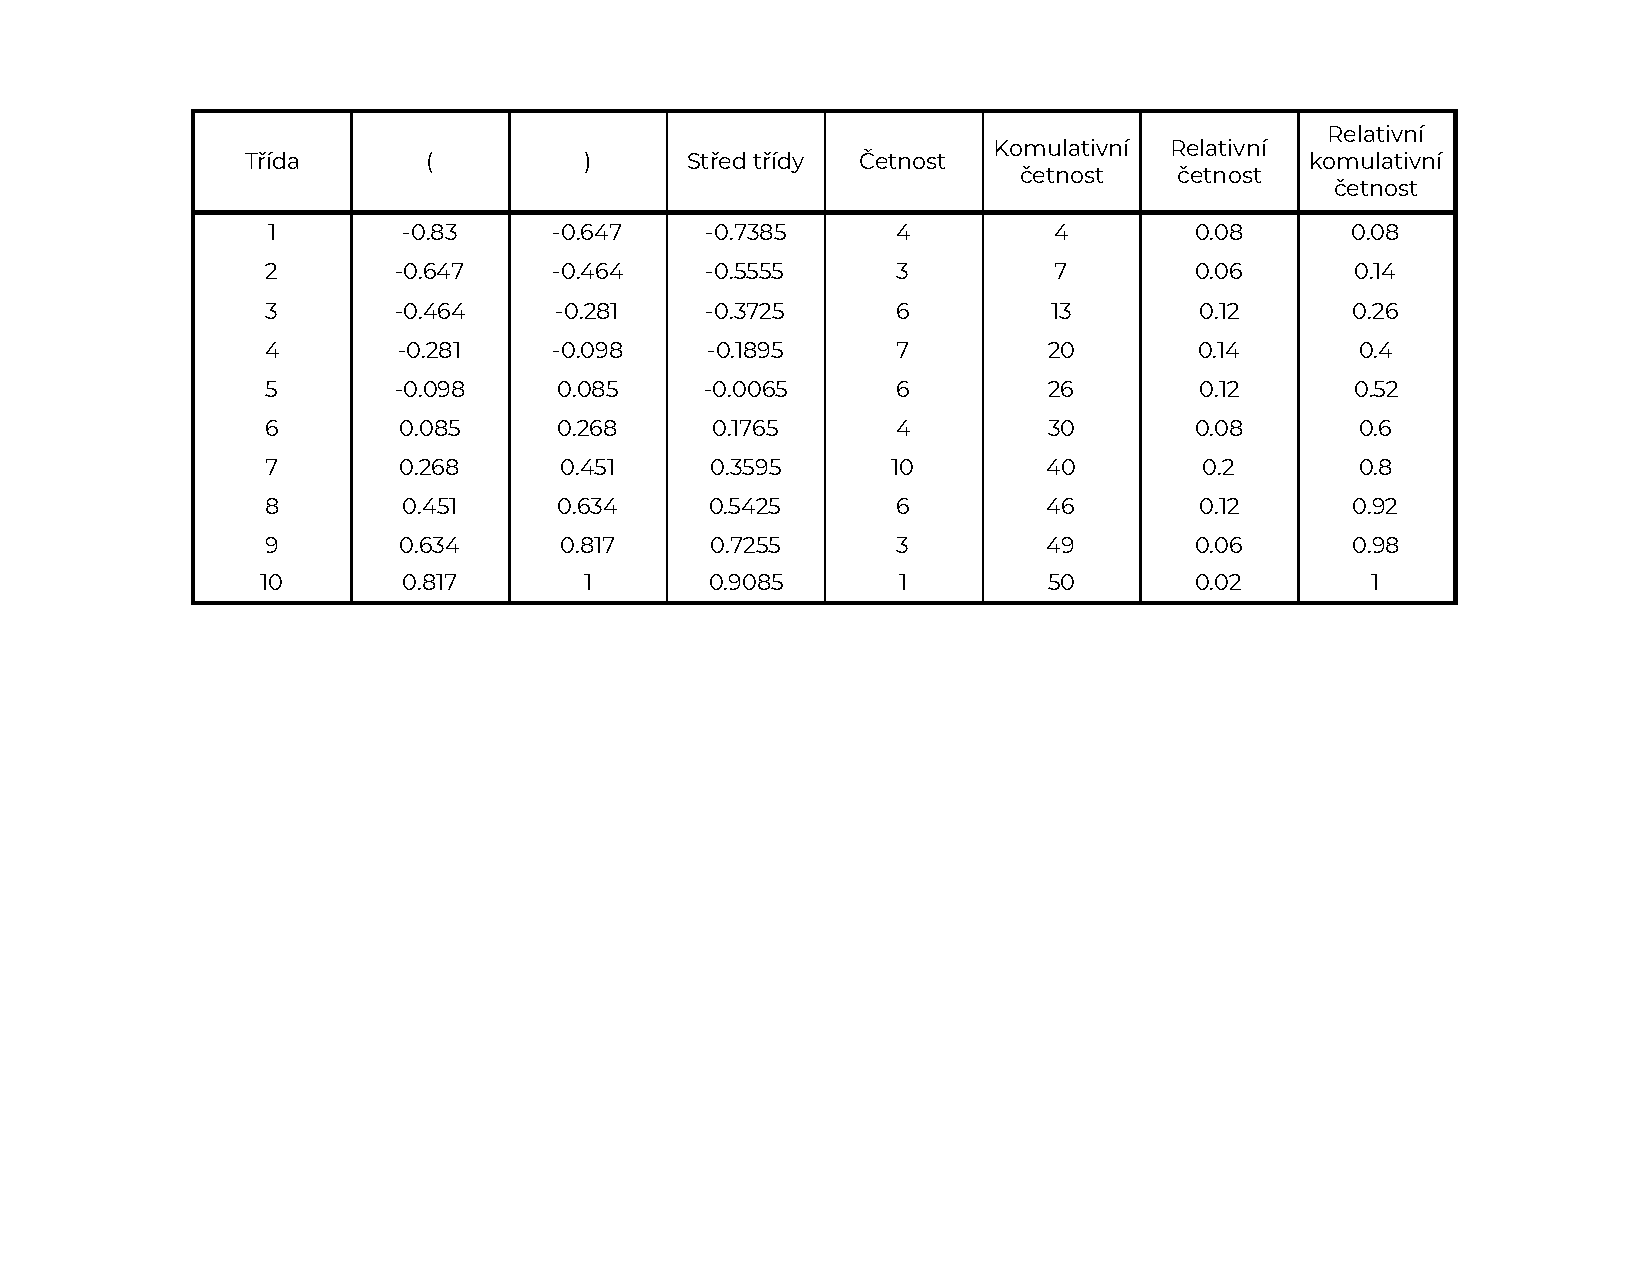
\includegraphics[width=1\linewidth]{1-a-1-crop.pdf}
\end{figure}

\begin{figure}[H]
    \centering
    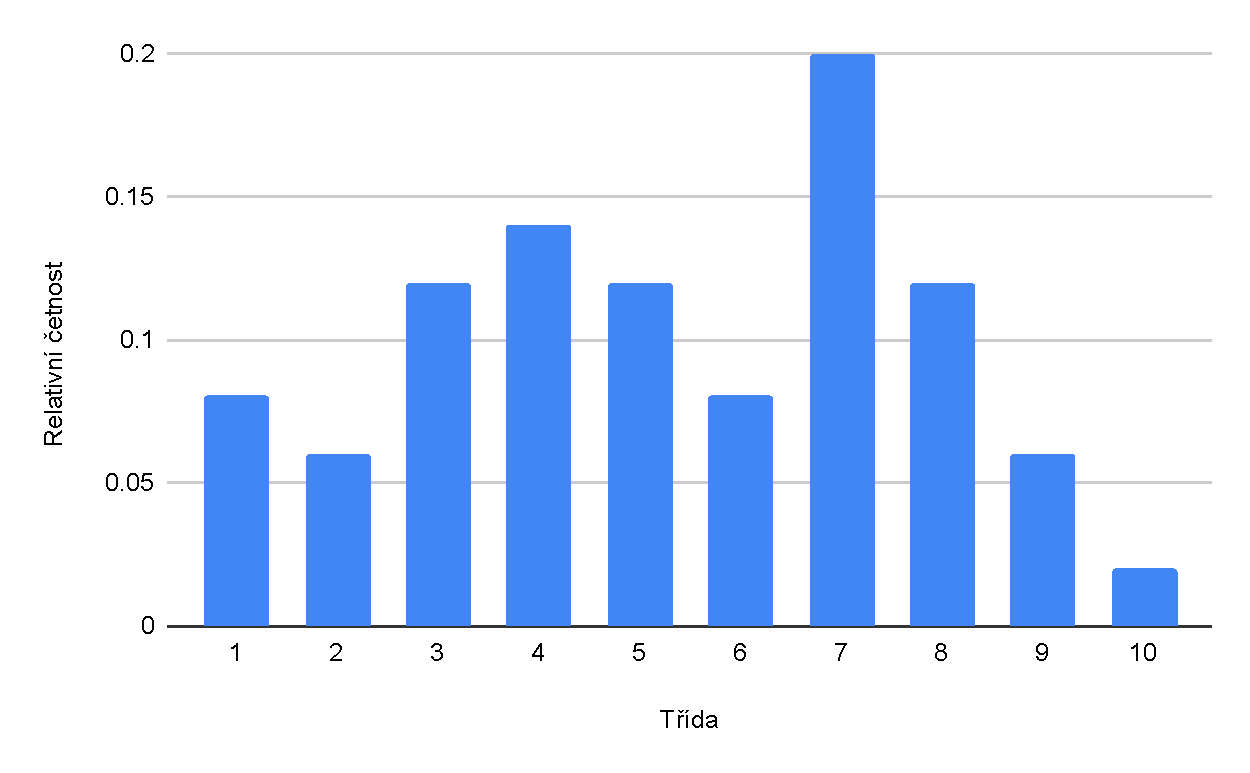
\includegraphics[width=.75\linewidth]{1-a-2.pdf}
\end{figure}

\begin{figure}[H]
    \centering
    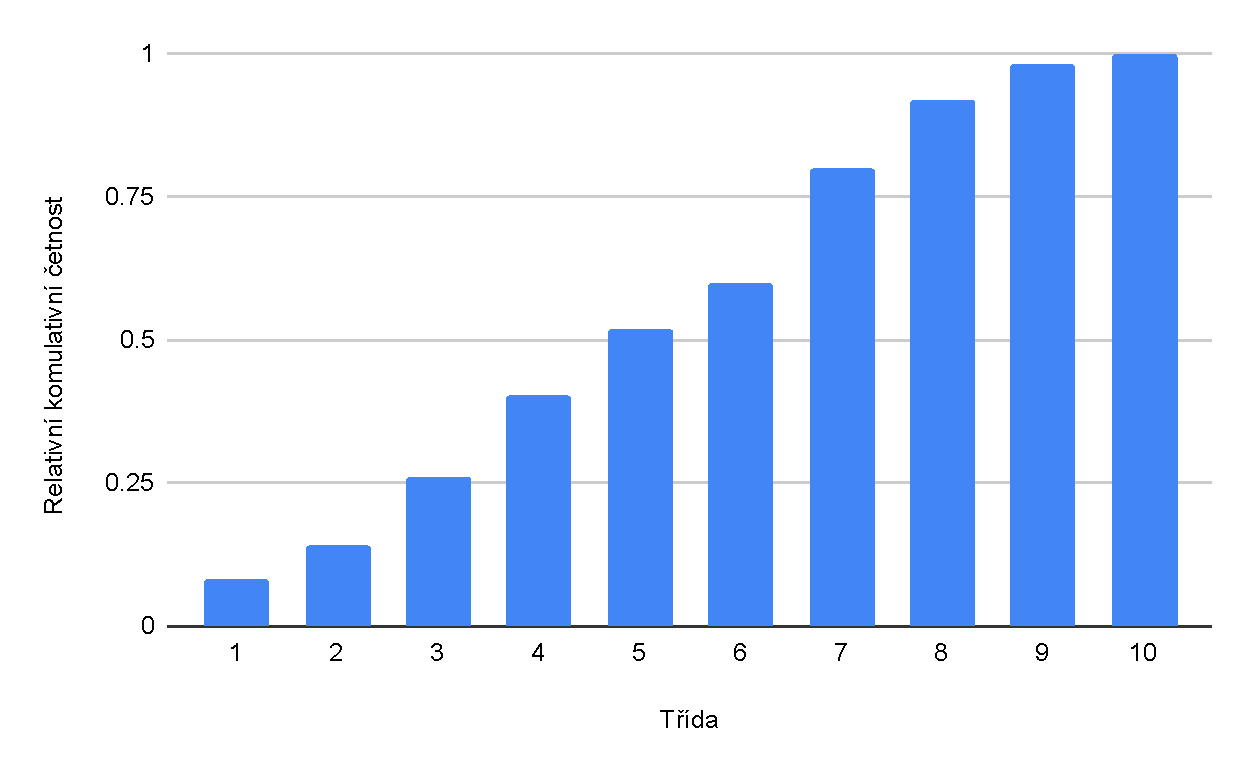
\includegraphics[width=.75\linewidth]{1-a-3.pdf}
\end{figure}

%%%%%%%%%%%%%%%%%%%%%%%%%%%%%%%%%%%%%%%%%%%%%%%%%%%%%%%%%%%%%%%%%%%%%

\subsection{Vypočtěte aritmetický průměr, medián, modus, rozptyl a směrodatnou odchylku.}

\begin{compactitem}
    \item Aritmetický průměr:
    $${\displaystyle \overline{x} = {\frac {1}{n}} \sum_{i=1}^{n} x_{i} = 0.0546}$$

    \item Medián:
    $${\displaystyle \tilde{x} = 0.075}$$

    \item Modus:
    $${\displaystyle \hat{x} = 0.44}$$

    \item Rozptyl:
    $${\displaystyle s^2 = {\frac {1}{n}} \sum_{i=1}^{n}(x_i - \overline{x})^2} \approx 0.2031$$

    \item Směrodatná odchylka:
    $${\displaystyle s = \sqrt{{\frac {1}{n}} \sum_{i=1}^{n}(x_i - \overline{x})^2}} \approx 0.4507$$
\end{compactitem}

%%%%%%%%%%%%%%%%%%%%%%%%%%%%%%%%%%%%%%%%%%%%%%%%%%%%%%%%%%%%%%%%%%%%%

\subsection{Vypočtěte bodové odhady střední hodnoty, rozptylu a směrodatné odchylky.}

\begin{compactitem}
    \item Bodový odhad střední hodnoty:
    $${\displaystyle \overline{x} = {\frac {1}{n}} \sum_{i=1}^{n} x_{i} = 0.0546}$$

    \item Bodový odhad rozptylu:
    $${\displaystyle s^2 = {\frac {1}{n-1}} \sum_{i=1}^{n}(x_i - \overline{x})^2} \approx 0.2073$$

    \item Bodový odhad směrodatné odchylky:
    $${\displaystyle s = \sqrt{{\frac {1}{n-1}} \sum_{i=1}^{n}(x_i - \overline{x})^2}} \approx 0.4553$$
\end{compactitem}

%%%%%%%%%%%%%%%%%%%%%%%%%%%%%%%%%%%%%%%%%%%%%%%%%%%%%%%%%%%%%%%%%%%%%

\subsection{Testujte předpoklad o výběru z normálního rozdělení Pearsonovým (chí-kvadrát) testem na hladině významnosti $0.05$.}

\begin{figure}[H]
    \centering
    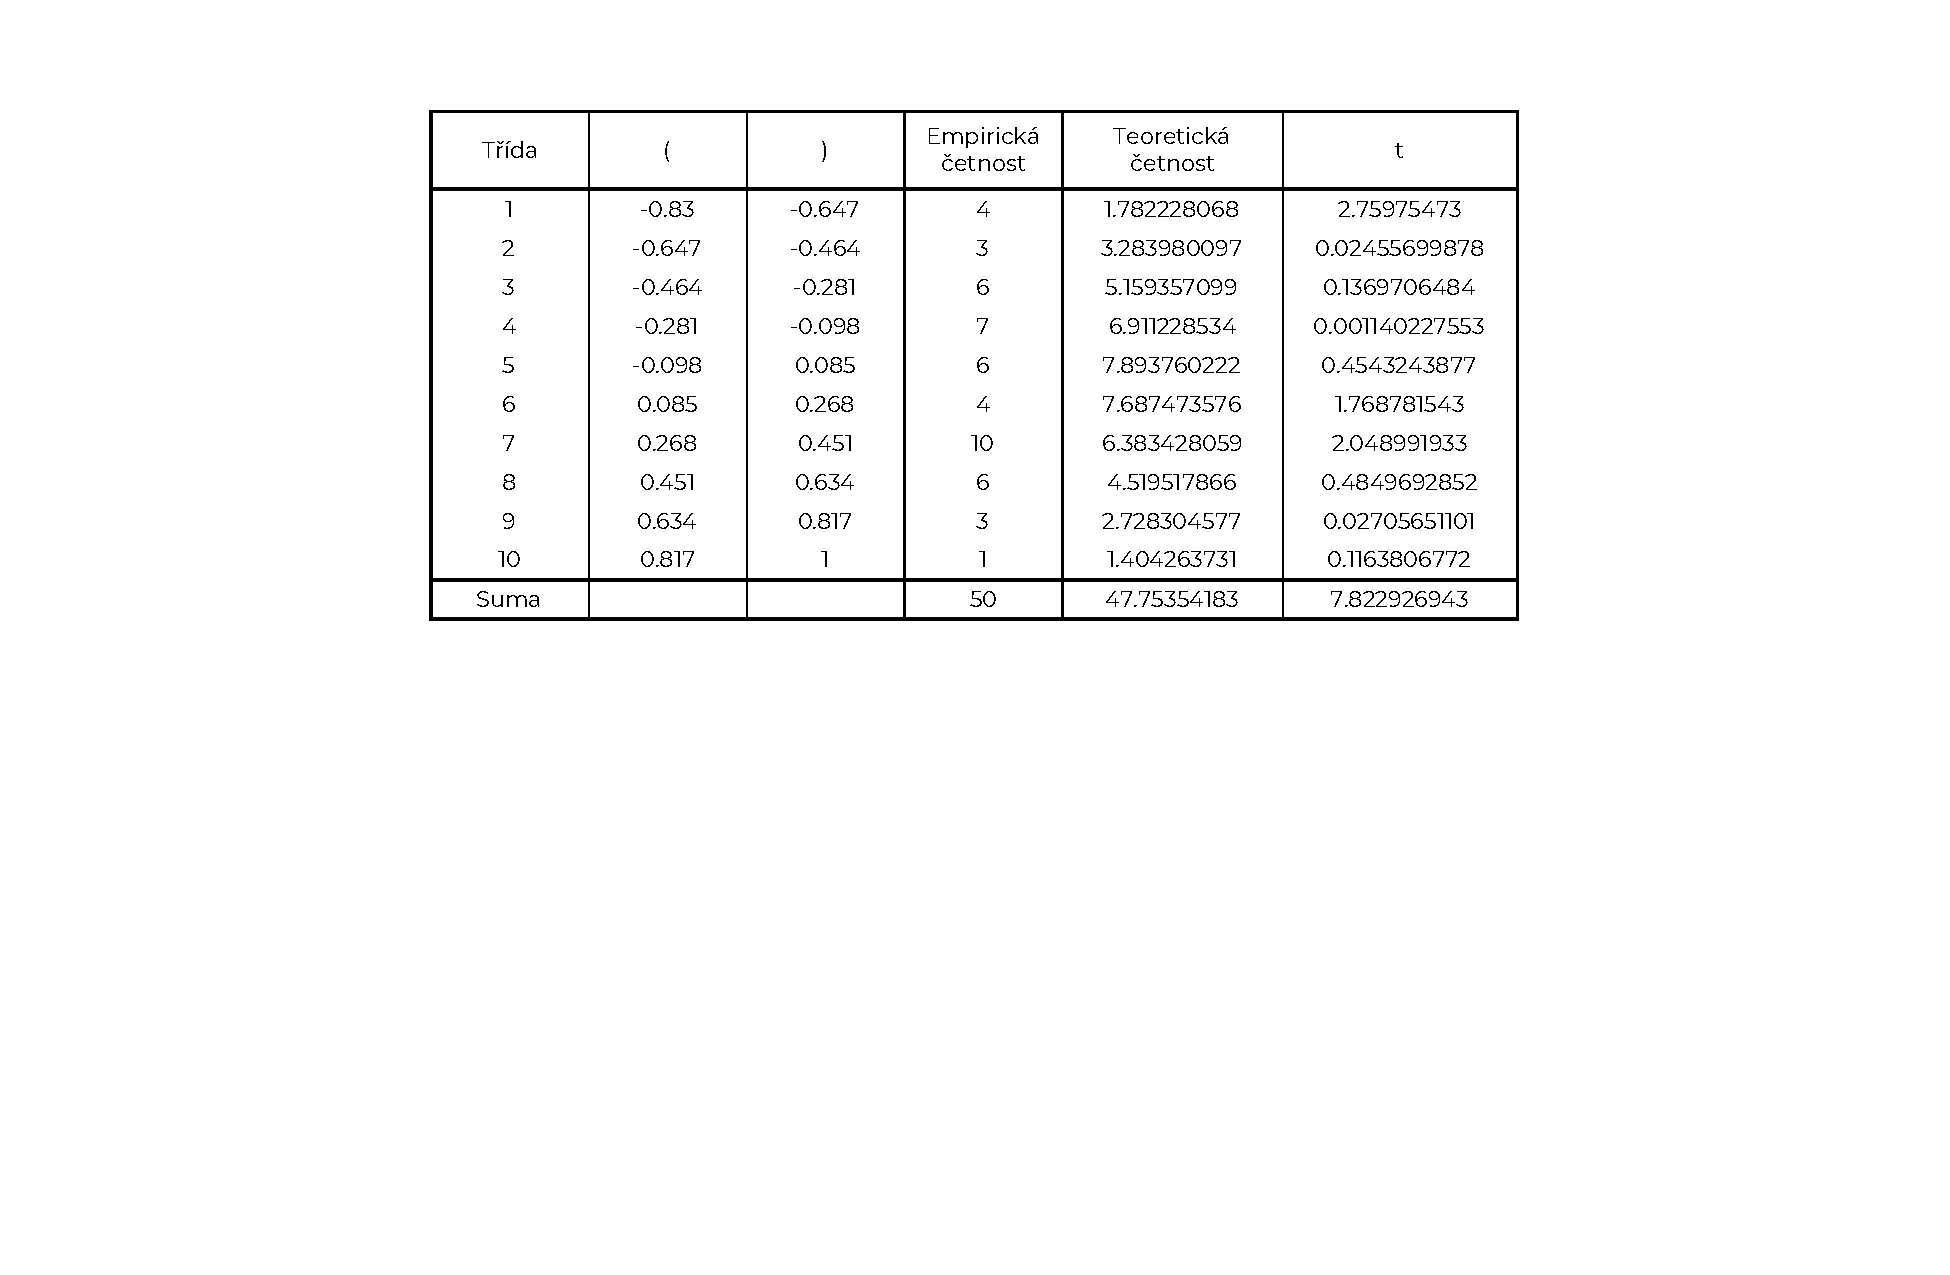
\includegraphics[width=1\linewidth]{1-d-1-crop.pdf}
\end{figure}

\begin{compactitem}
    \item Aby celkový počet teoretických četností odpovídal reálným, byly krajní intervaly rozšířeny. Aby všechny teoretické četnosti byly větší jako 1 a aspoň 80\,\% z nich bylo větších než 5 byly hranice tříd upraveny.
\end{compactitem}

\begin{figure}[H]
    \centering
    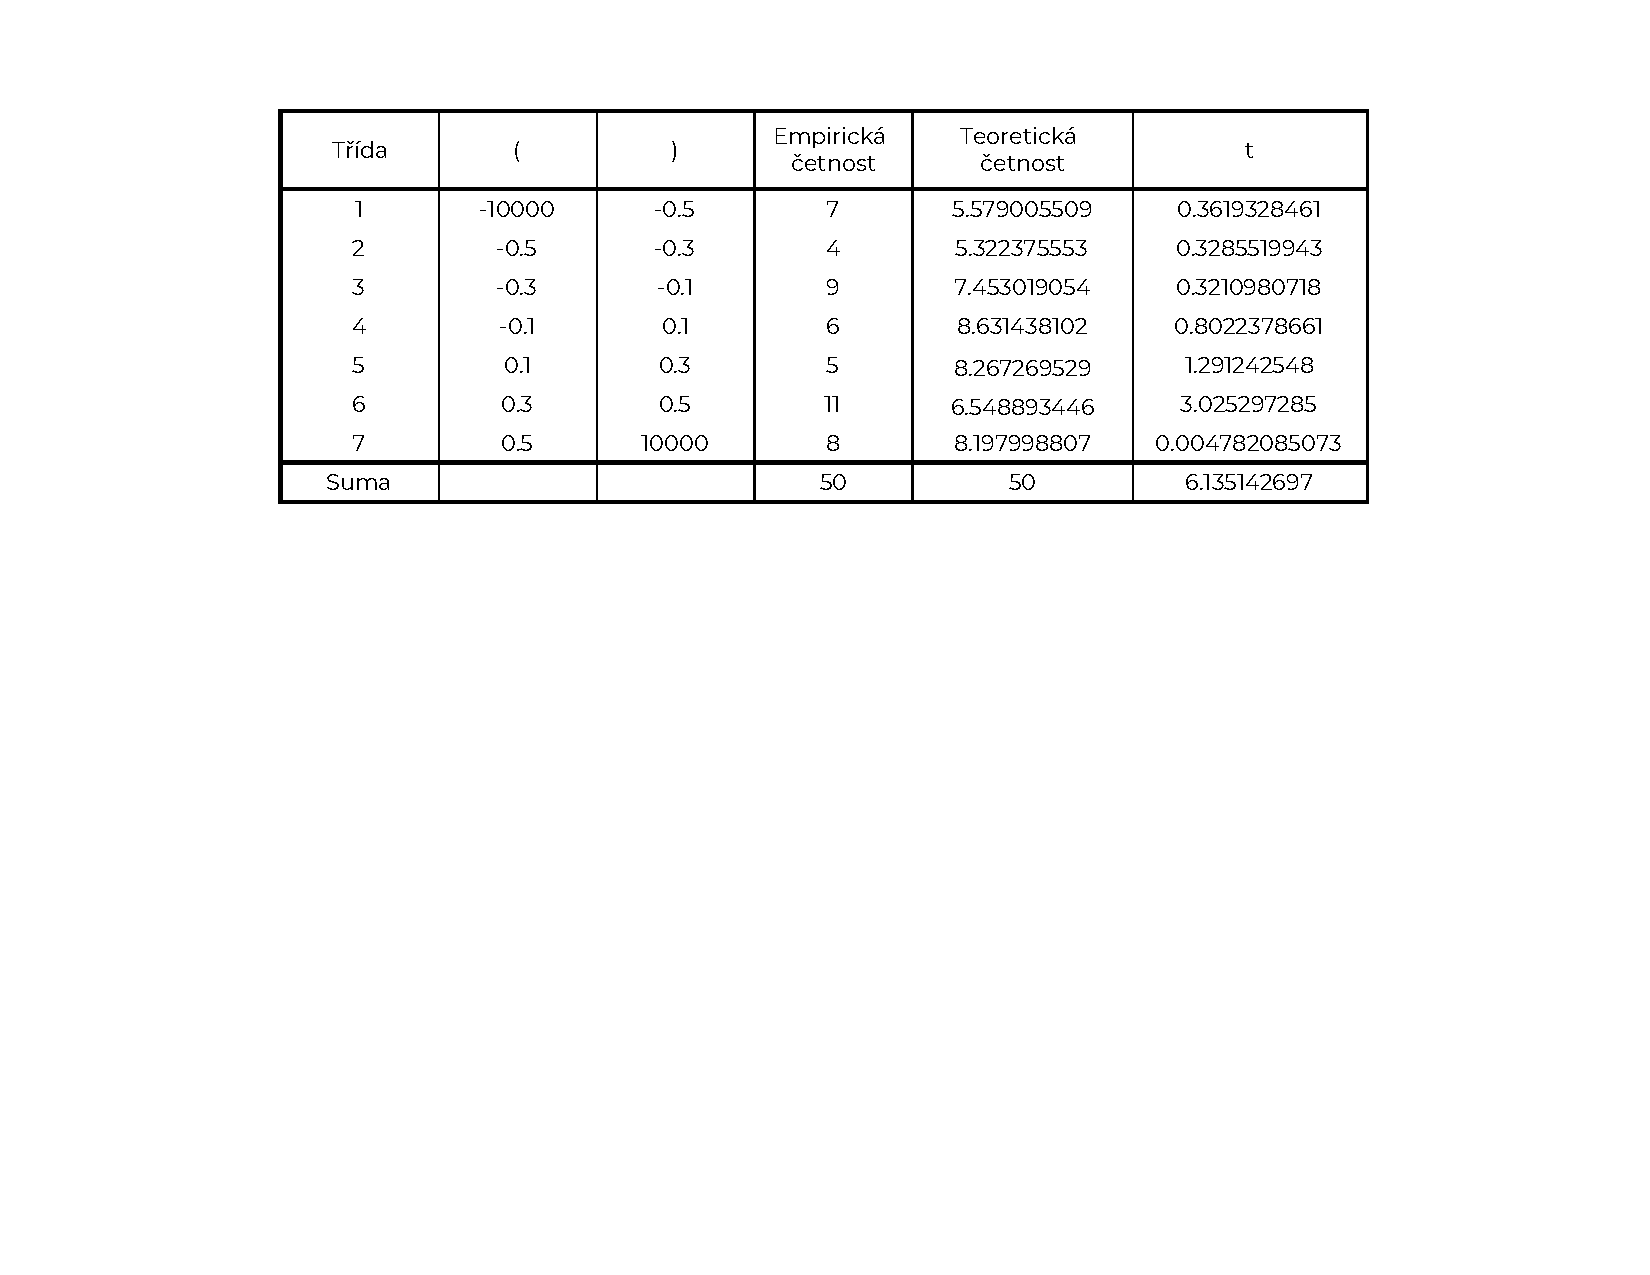
\includegraphics[width=1\linewidth]{1-d-2-crop.pdf}
\end{figure}

\begin{compactitem}
    \item Testovací kritérium: ${\displaystyle t = \sum_{i=1}^{m} = \frac{(f_i - \hat{f_i})^2}{\hat{f_i}} \approx 6.135}$, kde $f$ je empirická četnost a $\hat{f}$ je teoretická četnost.

    \item Stupeň volnosti: ${\displaystyle k = m - q - 1 = 4}$, kde $m$ je počet tříd a $q$ je počet odhadů parametrů.

    \item Kvantil Pearsonova rozdělení pro hladinu významnosti ${\displaystyle \alpha = 0.05}$:
    $${\displaystyle \qquad \chi_{1 - \alpha}^2(k) = \chi_{0.95}^2(4) \approx 9.4877}$$

    \item Doplněk kritického oboru:
    $${\displaystyle \overline{W_\alpha} = \big\langle 0 ~,~ \chi_{1 - \alpha}^2(k) \big\rangle \approx \big\langle 0 ~,~ 9.4877 \big\rangle}$$

    \item Jelikož ${\displaystyle t \in \overline{W_\alpha}}$, tak hypotéza ${\displaystyle X \sim N(0.0546, 0.2073)}$ se \textbf{nezamítá}.
\end{compactitem}

\begin{figure}[H]
    \centering
    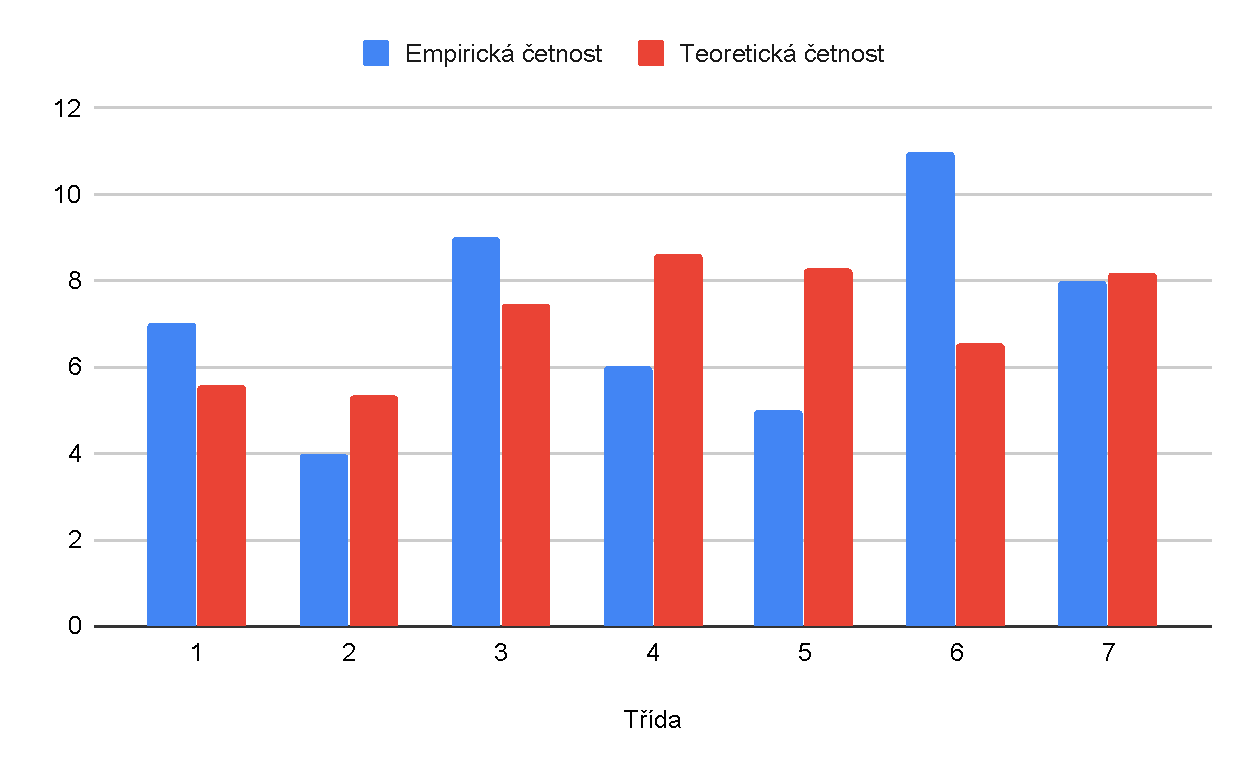
\includegraphics[width=1\linewidth]{1-d-3.pdf}
\end{figure}

%%%%%%%%%%%%%%%%%%%%%%%%%%%%%%%%%%%%%%%%%%%%%%%%%%%%%%%%%%%%%%%%%%%%%

\subsection{Za předpokladu (bez ohledu na výsledek části d), že statistický soubor byl získán náhodným výběrem z normálního rozdělení, určete intervalové odhady střední hodnoty, rozptylu a směrodatné odchylky se spolehlivostí $0.95$ a $0.99$.}

\begin{compactitem}
    \item Předpokládáme ${\displaystyle X \sim N(\mu, \sigma^2)}$

    \item Bodový odhad střední hodnoty: ${\displaystyle \overline{x} = 0.0546}$

    \item Bodový odhad rozptylu: ${\displaystyle s^2 \approx 0.2073}$

    \item Bodový odhad směrodatné odchylky: ${\displaystyle s \approx 0.4553}$
\end{compactitem}

\paragraph*{Intervalový odhad střední hodnoty}

\begin{compactitem}
    \item Stupeň volnosti: ${\displaystyle k = n - 1 = 49}$, kde $n$ je počet vzorků.

    \item Kvantil Studentova rozdělení pro hladinu významnosti ${\displaystyle \alpha = 0.05}$:
    $${\displaystyle \qquad t_{1 - \frac{\alpha}{2}}(k) = t_{0.975}(49) \approx 2.0096}$$

    \item Kvantil Studentova rozdělení pro hladinu významnosti ${\displaystyle \alpha = 0.01}$:
    $${\displaystyle \qquad t_{1 - \frac{\alpha}{2}}(k) = t_{0.995}(49) \approx 2.6799}$$

    \item Střední hodnota pro ${\displaystyle \alpha = 0.05 :}$
    $${\displaystyle \qquad \mu \in \bigg\langle \overline{x} - t_{1 - \frac{\alpha}{2}}(k) \cdot \frac{s}{\sqrt{n}} ~,~ \overline{x} + t_{1 - \frac{\alpha}{2}}(k) \cdot \frac{s}{\sqrt{n}} \bigg\rangle \approx \bigg\langle -0.0761 ~,~ 0.1853 \bigg\rangle}$$

    \item Střední hodnota pro ${\displaystyle \alpha = 0.01 :}$
    $${\displaystyle \qquad \mu \in \bigg\langle \overline{x} - t_{1 - \frac{\alpha}{2}}(k) \cdot \frac{s}{\sqrt{n}} ~,~ \overline{x} + t_{1 - \frac{\alpha}{2}}(k) \cdot \frac{s}{\sqrt{n}} \bigg\rangle \approx \bigg\langle -0.1197 ~,~ 0.2289 \bigg\rangle}$$
\end{compactitem}

\paragraph*{Intervalový odhad rozptylu}

\begin{compactitem}
    \item Kvantil Pearsonova rozdělení pro hladinu významnosti ${\displaystyle \alpha = 0.05}$:
    $${\displaystyle \qquad \chi_{\frac{\alpha}{2}}^2(k) = \chi_{0.025}^2(49) \approx 31.555}$$
    $${\displaystyle \qquad \chi_{1 - \frac{\alpha}{2}}^2(k) = \chi_{0.975}^2(49) \approx  70.222}$$

    \item Kvantil Pearsonova rozdělení pro hladinu významnosti ${\displaystyle \alpha = 0.01}$:
    $${\displaystyle \qquad \chi_{\frac{\alpha}{2}}^2(k) = \chi_{0.005}^2(49) \approx 27.249}$$
    $${\displaystyle \qquad \chi_{1 - \frac{\alpha}{2}}^2(k) = \chi_{0.995}^2(49) \approx  78.231}$$

    \item Rozptyl pro ${\displaystyle \alpha = 0.05 :}$
    $${\displaystyle \qquad \sigma^2 \in \bigg\langle \frac{(n - 1) \cdot s^2}{\chi_{1 - \frac{\alpha}{2}}^2(k)} ~,~ \frac{(n - 1) \cdot s^2}{\chi_{\frac{\alpha}{2}}^2(k)} \bigg\rangle \approx \bigg\langle 0.1447 ~,~ 0.3219 \bigg\rangle}$$

    \item Rozptyl pro ${\displaystyle \alpha = 0.01 :}$
    $${\displaystyle \qquad \sigma^2 \in \bigg\langle \frac{(n - 1) \cdot s^2}{\chi_{1 - \frac{\alpha}{2}}^2(k)} ~,~ \frac{(n - 1) \cdot s^2}{\chi_{\frac{\alpha}{2}}^2(k)} \bigg\rangle \approx \bigg\langle 0.1298 ~,~ 0.3727 \bigg\rangle}$$
\end{compactitem}

\paragraph*{Intervalový odhad směrodatné odchylky}

\begin{compactitem}
    \item Směrodatná odchylka pro ${\displaystyle \alpha = 0.05 :}$
    $${\displaystyle \qquad \sigma \in \bigg\langle \sqrt{\frac{(n - 1) \cdot s^2}{\chi_{1 - \frac{\alpha}{2}}^2(k)}} ~,~ \sqrt{\frac{(n - 1) \cdot s^2}{\chi_{\frac{\alpha}{2}}^2(k)}} \bigg\rangle \approx \bigg\langle 0.3803 ~,~ 0.5674 \bigg\rangle}$$

    \item Směrodatná odchylka pro ${\displaystyle \alpha = 0.01 :}$
    $${\displaystyle \qquad \sigma \in \bigg\langle \sqrt{\frac{(n - 1) \cdot s^2}{\chi_{1 - \frac{\alpha}{2}}^2(k)}} ~,~ \sqrt{\frac{(n - 1) \cdot s^2}{\chi_{\frac{\alpha}{2}}^2(k)}} \bigg\rangle \approx \bigg\langle 0.3603 ~,~ 0.6106 \bigg\rangle}$$
\end{compactitem}

%%%%%%%%%%%%%%%%%%%%%%%%%%%%%%%%%%%%%%%%%%%%%%%%%%%%%%%%%%%%%%%%%%%%%

\subsection{Testujte hypotézu optimálního seřízení stroje, tj. že střední hodnota odchylky je nulová, proti dvoustranné alternativní hypotéze, že střední hodnota odchylky je různá od nuly, a to na hladině významnosti $0.05$.}

\begin{compactitem}
    \item Hypotéza: ${\displaystyle H_0 : \mu = 0}$

    \item Alternativní hypotéza: ${\displaystyle H_{A} : \mu \neq 0}$

    \item Bodový odhad střední hodnoty: ${\displaystyle \overline{x} = 0.0546}$

    \item Bodový odhad směrodatné odchylky: ${\displaystyle s \approx 0.4553}$

    \item Počet vzorků: ${\displaystyle n = 50}$
\end{compactitem}

\paragraph*{Testujeme pomocí Studentova jednovýběrového testu}

\begin{compactitem}
    \item Testovací kritérium: ${\displaystyle t = \frac{\overline{x} - \mu}{s} \cdot \sqrt{n} \approx 0.848}$

    \item Stupeň volnosti: ${\displaystyle k = n - 1 = 49}$

    \item Kvantil Studentova rozdělení pro hladinu významnosti ${\displaystyle \alpha = 0.05}$:
    $${\displaystyle \qquad t_{1 - \frac{\alpha}{2}}(k) = t_{0.975}(49) \approx 2.0096}$$

    \item Doplněk kritického oboru pro alternativní hypotézu ${\displaystyle H_{A}}$:
    $${\displaystyle \qquad \overline{W_\alpha} = \big\langle -t_{1 - \frac{\alpha}{2}}(k) ~,~ t_{1 - \frac{\alpha}{2}}(k) \big\rangle \approx \big\langle -2.0096 ~,~ 2.0096 \big\rangle}$$

    \item Jelikož ${\displaystyle t \in \overline{W_\alpha}}$, tak hypotéza ${\displaystyle H_0}$ se \textbf{nezamítá} a alternativní hypotéza ${\displaystyle H_A}$ se \textbf{zamítá}.
\end{compactitem}

%%%%%%%%%%%%%%%%%%%%%%%%%%%%%%%%%%%%%%%%%%%%%%%%%%%%%%%%%%%%%%%%%%%%%

\subsection{Ověřte statistickým testem na hladině významnosti $0.05$, zda seřízení stroje ovlivnilo kvalitu výroby, víte-li, že výše uvedený statistický soubor $50$ hodnot vznikl spojením dvou dílčích statistických souborů tak, že po naměření prvních $20$ hodnot bylo provedeno nové seřízení stroje a pak bylo naměřeno zbývajících $30$ hodnot.}

\begin{figure}[H]
    \centering
    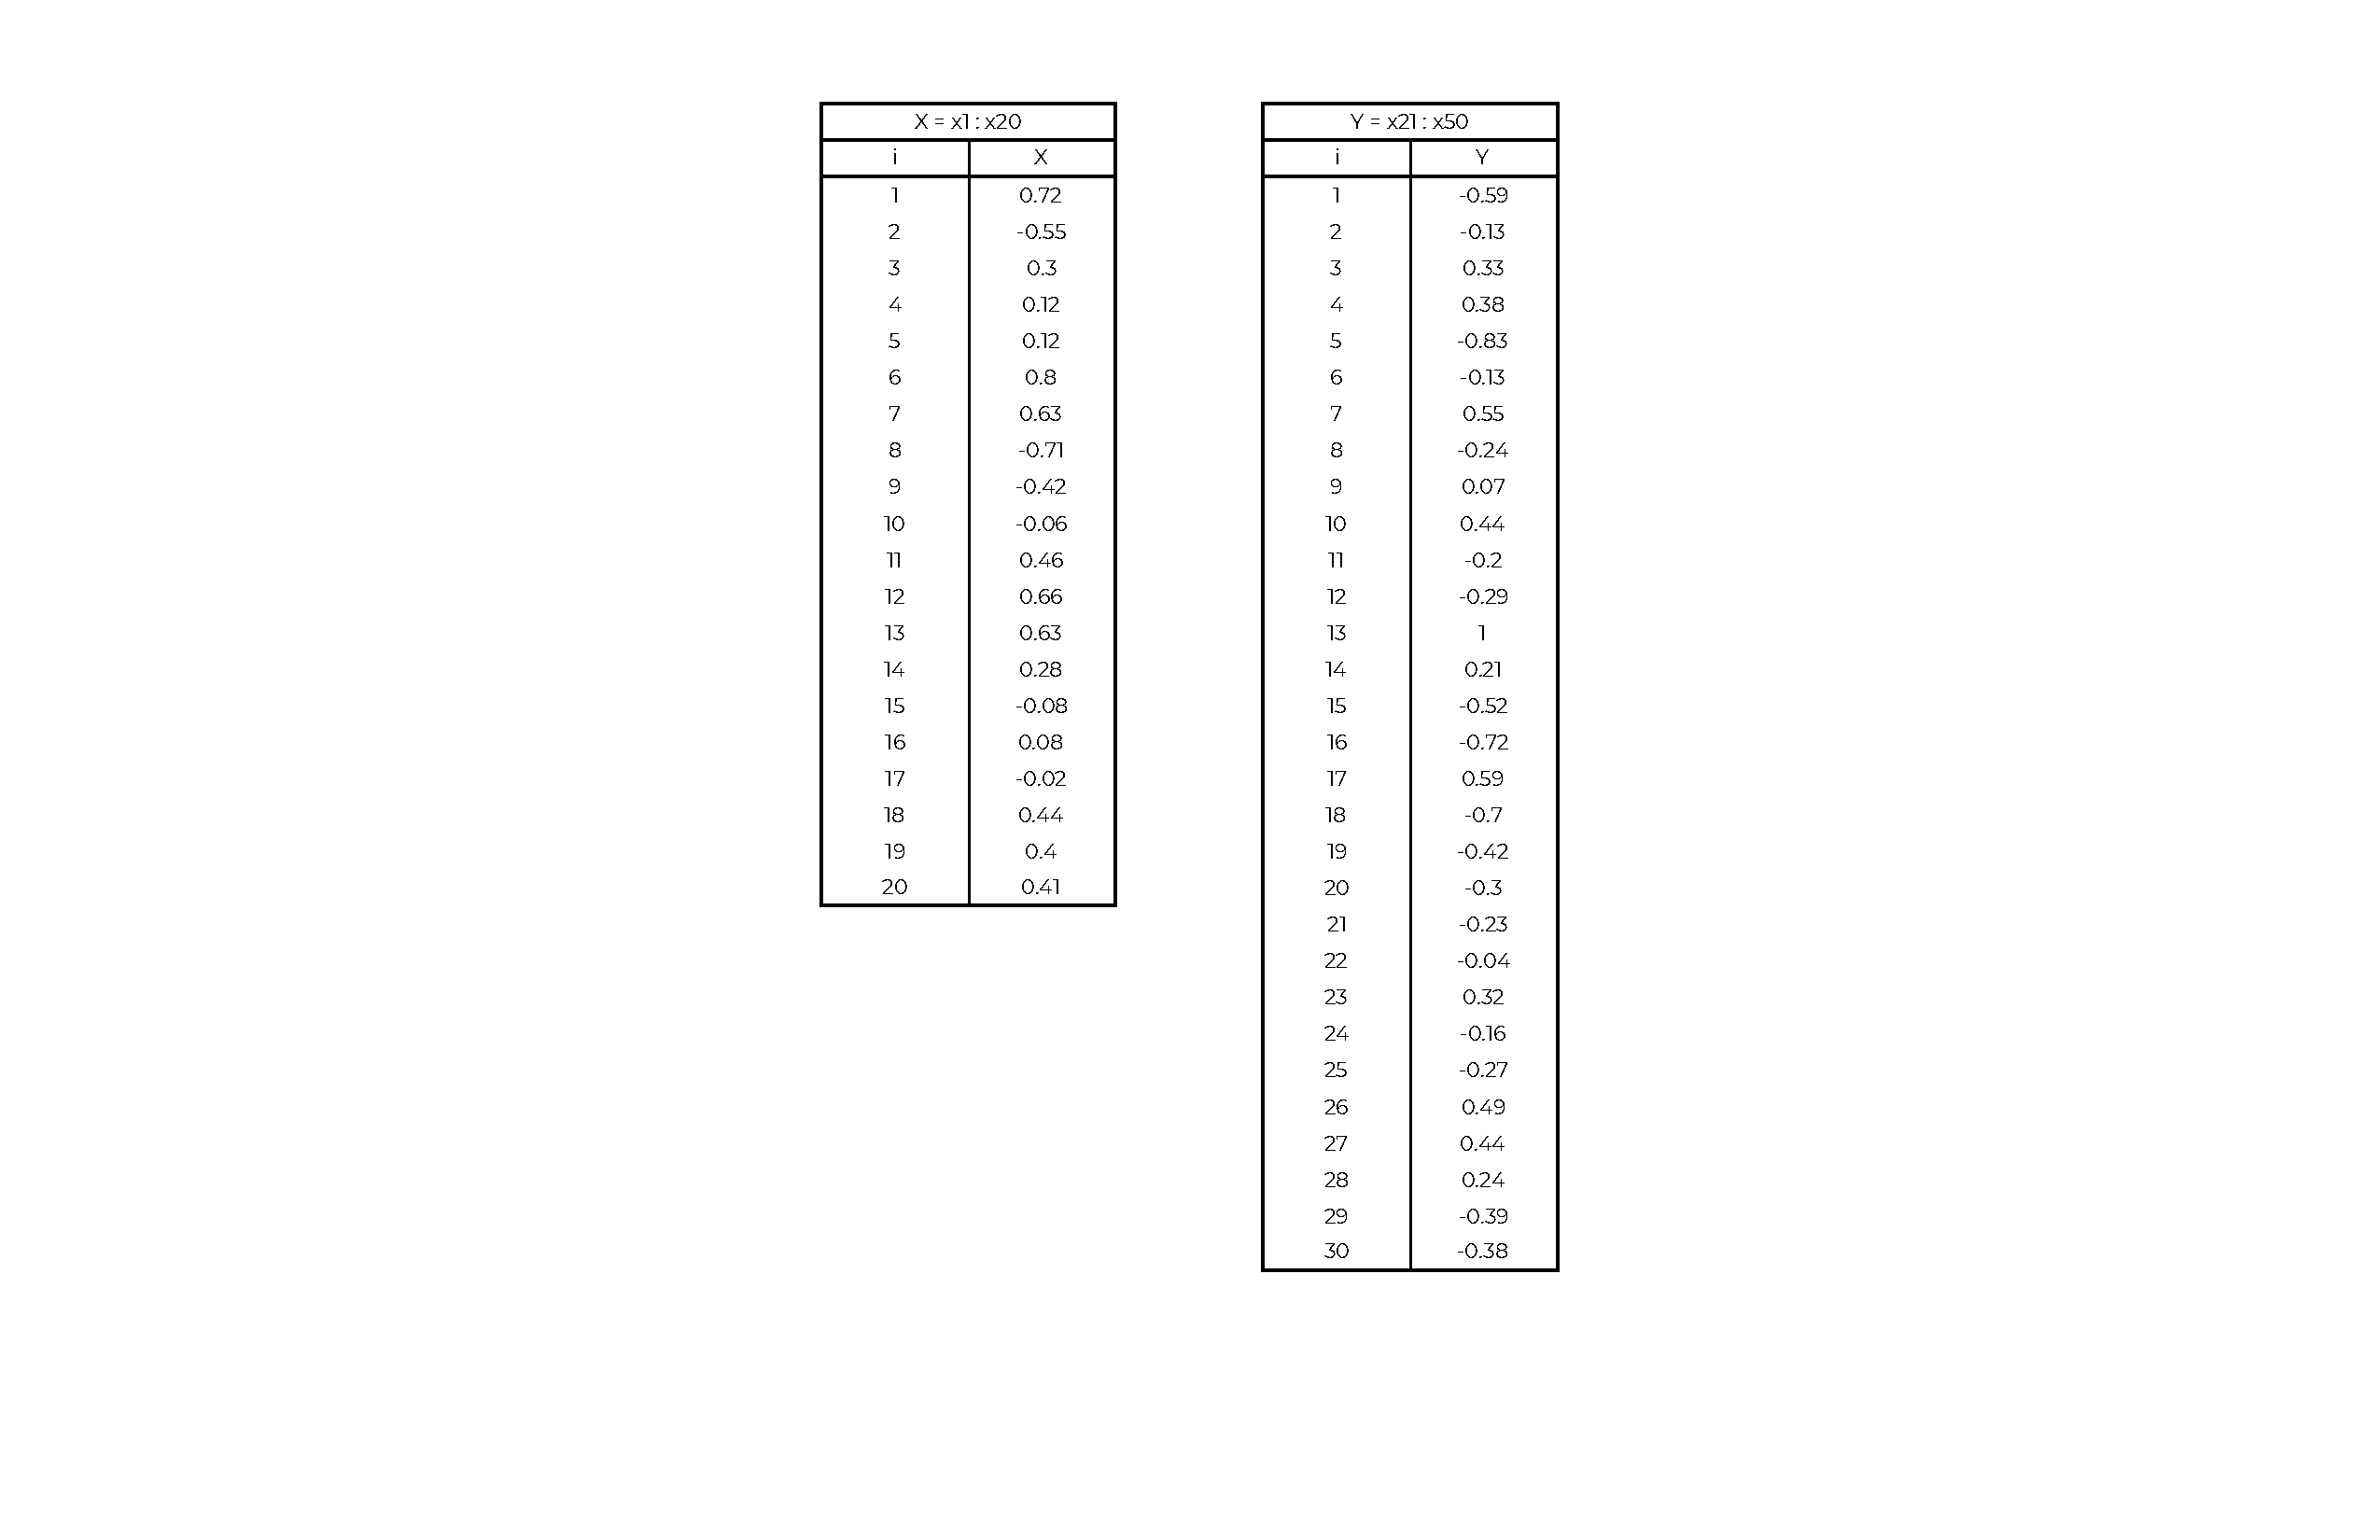
\includegraphics[width=.7\linewidth]{1-g-1-crop.pdf}
\end{figure}

\begin{minipage}{0.49\textwidth}
    $${\displaystyle n_x = 20}$$
    $${\displaystyle \overline{x} = 0.2105}$$
    $${\displaystyle s_x^2 \approx 0.1806}$$
    $${\displaystyle s_x \approx 0.425}$$
\end{minipage}
%
\begin{minipage}{0.49\textwidth}
    $${\displaystyle n_y = 30}$$
    $${\displaystyle \overline{y} \approx -0.0493}$$
    $${\displaystyle s_y^2 \approx 0.2039}$$
    $${\displaystyle s_y \approx 0.4516}$$
\end{minipage}

\paragraph*{Test rovnosti rozptylů pomocí F-testu}

\begin{compactitem}
    \item Hypotéza
    $${\displaystyle H_0 : \sigma_x^2 = \sigma_y^2}$$

    \item  Alternativní hypotéza
    $${\displaystyle H_A : \sigma_x^2 \neq \sigma_y^2}$$

    \item  Testovací kritérium:
    $${\displaystyle t = \frac{s_x^2}{s_y^2} \approx 0.7844}$$

    \item Stupně volnosti:
    $${\displaystyle \qquad k_x = n_x - 1 = 19}$$
    $${\displaystyle \qquad k_y = n_y - 1 = 29}$$

    \item Kvantily Fisher-Snedecorova rozdělení pro hladinu významnosti ${\displaystyle \alpha = 0.05}$:
    $${\displaystyle \qquad F_{\frac{\alpha}{2}} (k_x, k_y) = F_{0.025} (19, 29) \approx 0.4163}$$
    $${\displaystyle \qquad F_{1 - \frac{\alpha}{2}} (k_x, k_y) = F_{0.975} (19, 29) \approx 2.2313}$$

    \item  Doplněk kritického oboru pro alternativní hypotézu ${\displaystyle H_A}$:
    $${\displaystyle \qquad \overline{W_\alpha} = \big\langle F_{\frac{\alpha}{2}} (k_x, k_y) ~,~ F_{1 - \frac{\alpha}{2}} (k_x, k_y) \big\rangle \approx \big\langle 0.4163 ~,~ 2.2313 \big\rangle}$$

    \item Jelikož ${\displaystyle t \in \overline{W_\alpha}}$, tak hypotéza ${\displaystyle H_0}$ se \textbf{nezamítá}.
\end{compactitem}

\paragraph*{Test rovnosti středních hodnot pomocí Studentova dvouvýběrového testu}

\begin{compactitem}
    \item Hypotéza (pro ${\displaystyle \mu_0 = 0}$ za podmínky ${\displaystyle \sigma_x^2 = \sigma_y^2}$)
    $${\displaystyle H_0 : \mu_x - \mu_y = \mu_0}$$

    \item Alternativní hypotéza
    $${\displaystyle H_A : \mu_x - \mu_y \neq 0}$$

    \item Stupeň volnosti:
    $${\displaystyle k = n_x + n_y -2 = 48}$$

    \item Testovací kritérium:
    $${\displaystyle t = \frac{\overline{x} - \overline{y} - \mu_0}{\sqrt{k_x \cdot s_x^2 + k_y \cdot s_y^2}} \cdot \sqrt{\frac{n_x \cdot n_y \cdot k}{n_x + n_y}} \approx 2.04}$$

    \item Kvantil Studentova rozdělení pro hladinu významnosti ${\displaystyle \alpha = 0.05}$:
    $${\displaystyle \qquad t_{1 - \frac{\alpha}{2}}(k) = t_{0.975}(48) \approx 2.0106}$$

    \item Doplněk kritického oboru pro alternativní hypotézu ${\displaystyle H_{A}}$:
    $${\displaystyle \qquad \overline{W_\alpha} = \big\langle -t_{1 - \frac{\alpha}{2}}(k) ~,~ t_{1 - \frac{\alpha}{2}}(k) \big\rangle \approx \big\langle -2.0106 ~,~ 2.0106 \big\rangle}$$

    \item Jelikož ${\displaystyle t \notin \overline{W_\alpha}}$, tak hypotéza ${\displaystyle H_0}$ se \textbf{zamítá}.
\end{compactitem}
